\documentclass{article}
\usepackage{tkz-graph}
\usepackage{paralist}
\pagestyle{empty}
\usetikzlibrary{patterns}

\begin{document}

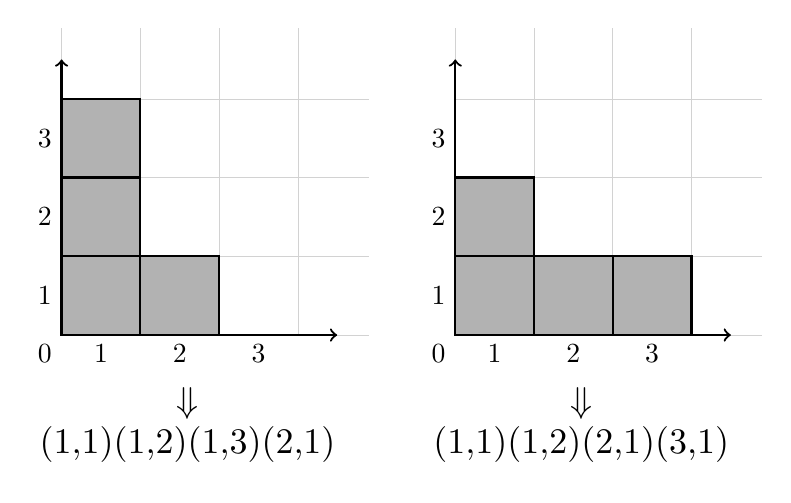
\begin{tikzpicture}
\draw[step=1cm,gray!35,very thin] (0,0) grid (3.9,3.9);

\draw[thick,->] (0,0) -- (3.5,0);
\draw[thick,->] (0,0) -- (0,3.5);

\draw (0,0) node[anchor=north east] {0};
\draw (0.5,0) node[anchor=north] {1};
\draw (1.5,0) node[anchor=north] {2};
\draw (2.5,0) node[anchor=north] {3};
\draw (0,0.5) node[anchor=east] {1};
\draw (0,1.5) node[anchor=east] {2};
\draw (0,2.5) node[anchor=east] {3};

\filldraw[gray!60, draw=black, thick] (0,0) rectangle (1,1);
\filldraw[gray!60, draw=black, thick] (0,1) rectangle (1,2);
\filldraw[gray!60, draw=black, thick] (0,2) rectangle (1,3);
\filldraw[gray!60, draw=black, thick] (1,0) rectangle (2,1);

\draw (1.6,-0.5) node[anchor=north, scale=1.3] {$\Downarrow$};
\draw (1.6,-1) node[anchor=north, scale=1.3] {(1,1)(1,2)(1,3)(2,1)};

\draw[step=1cm,gray!35,very thin] (5,0) grid (8.9,3.9);

\draw[thick,->] (5,0) -- (8.5,0);
\draw[thick,->] (5,0) -- (5,3.5);

\draw (5,0) node[anchor=north east] {0};
\draw (5.5,0) node[anchor=north] {1};
\draw (6.5,0) node[anchor=north] {2};
\draw (7.5,0) node[anchor=north] {3};
\draw (5,0.5) node[anchor=east] {1};
\draw (5,1.5) node[anchor=east] {2};
\draw (5,2.5) node[anchor=east] {3};

\filldraw[gray!60, draw=black, thick] (5,0) rectangle (6,1);
\filldraw[gray!60, draw=black, thick] (5,1) rectangle (6,2);
\filldraw[gray!60, draw=black, thick] (6,0) rectangle (7,1);
\filldraw[gray!60, draw=black, thick] (7,0) rectangle (8,1);

\draw (6.6,-0.5) node[anchor=north, scale=1.3] {$\Downarrow$};
\draw (6.6,-1) node[anchor=north, scale=1.3] {(1,1)(1,2)(2,1)(3,1)};

\end{tikzpicture}

\end{document}